%% !TeX program = lualatex

%%%%%%%%%%%%%%%%%%%%%%%%%%%%%%%%%%%%%%%%%%%%%%%%%%%%%%%%%
% Niniejszy plik przedstawia przykładowy skład 
% pracy dyplomowej na Wydziale Matematyki PWr. 
% 
%
%%%%%%%%%%%%%%%%%%%%%%%%%%%%%%%%%%%%%%%%%%%%%%%%%%%%%%%%%
% Domyślną opcją jest: praca magisterska, język polski.
% W przypadku pracy pisanej w języku angielskim dodajemy 
% opcję [english].
% Dla pracy licencjackiej dodajemy opcję [licencjacka].
% Dla pracy inżynierskiej dodajemy opcję [inzynierska].
% Dopuszczalne są podwójne opcje, np. [licencjacka, english].
% Opcje dodajemy w kwadratowym nawiasie przy \documentclass.
%
%
%%%%%%%%%%%%%%%%%%%%%%%%%%%%%%%%%%%%%%%%%%%%%%%%%%%%%%%%%
\documentclass[english]{pwr_wmat_praca_dyplomowa}
%%%%%%%%%%%%%%%%%%%%%%%%%%%%%%%%%%%%%%%%%%%%%%%%%%%%%%%%%
%              DANE DO PRACY
%
% W przypadku pracy dyplomowej w języku angielskim nie jest konieczne 
% wypełnianie pól: \tytul{}, \kierunek{}, \specjalnosc{}, 
%                  \streszczenie{}, \slowakluczowe{}.
%%%%%%%%%%%%%%%%%%%%%%%%%%%%%%%%%%%%%%%%%%%%%%%%%%%%%%%%%
%
% Imię i nazwisko autora
\autor{Magdalena Wolniaczyk}
%
% Tytuł pracy dyplomowej 
% \tytul{Tytuł pracy dyplomowej} 
\tytulang{Comparison of Cognitive Diagnosis Models}
%
% Tytuł / stopień / imię i nazwisko opiekuna
\opiekun{Dr inż. Andrzej Giniewicz}
%
% Kierunek studiów wybieramy spośród następujących:
% 1) Matematyka
% 2) Matematyka i Statystyka
% 3) Matematyka stosowana
% \kierunekstudiow{Matematyka}
%
% Kierunek studiów po angielsku wybieramy spośród następujących:
% 1) Mathematics
% 2) Mathematics and Statistics
% 3) Applied Mathematics
\kierunekstudiowang{Applied Mathematics}
%
% Specjalność wybieramy spośród następujących: 
% KIERUNEK: Matematyka
% 1) Matematyka teoretyczna,
% 2) Statystyka matematyczna,
% 3) Matematyka finansowa i ubezpieczeniowa,
%
% KIERUNEK: Matematyka i Statystyka
% 4) Matematyka,
% 5) Statystyka i analiza danych, 
%
% 6) -- (w przypadku braku specjalizacji).
% \specjalnosc{Matematyka teoretyczna} 
%
% Specjalność w języku angielskim wybieramy spośród następujących:
% KIERUNEK: Matematyka
% 1) Theoretical Mathematics,
% 2) Mathematical Statistics,
% 3) Financial and Actuarial Mathematics,
%
% KIERUNEK: Matematyka i Statystyka
% 4) Mathematics,
% 5) Statistics and Data Analysis,
%
% KIERUNEK: Applied Mathematics
% 6) Financial and Actuarial Mathematics, 
% 7) Mathematics for Industry and Commerce,
% 8) Computational Mathematics,
% 9) Modelling, Simulation and Optimization.
%
% 10) -- (w przypadku braku specjalizacji).
\specjalnoscang{Data Engineering} 
%
% Krótkie streszczenia po polsku i angielsku
% - nie dłuższe niż 530 znaków.
% \streszczenie{Tutaj piszemy krótkie streszczenie pracy (nie powinno być dłuższe niż 530 znaków).}
\streszczenieang{Cognitive Diagnosis Models are one of the tools of mathematical cognitive psychology. Those models allow researchers to measure the skills of people based on some test results. The traits are described by latent variables. The test usually has dichotomous answers, which are linked to latent variables through a design matrix called the $Q$-matrix. The aim of this thesis is to compare commonly used models and to measure how robust they are. Furthermore, a simulation study will be conducted, to measure the effect of $Q$-matrix misspecification. Analysis of the real data set will be attempted as well.}
%
% Podajemy najważniejsze słowa kluczowe po polsku i angielsku
% - w obu przypadkach, nie więcej niż 150 znaków.
% \slowakluczowe{tutaj podajemy najważniejsze słowa kluczowe (łącznie nie powinny być dłuższe niż 150 znaków).}  
\slowakluczoweang{cognitive diagnosis models, $Q$-matrix, DINA, DINO, NIDA, G-NIDA, validation, robustness}
%
%
%%%%%%%%%%%%%%%%%%%%%%%%%%%%%%%%%%%%%%%%%%%%%%%%%%%%%%%%%
% Definicje, lematy, twierdzenia, przykłady i wnioski
% Komendy wywołujące twierdzenia, definicje, itd., 
% czyli 'theorem', 'definition', 'corollary', itd., 
% można zmienić wedle uznania.
\theoremstyle{plain}
\newtheorem{theorem}{Twierdzenie}
%\numberwithin{theorem}{chapter}
\newtheorem{lemma}[theorem]{Lemma} 
\newtheorem{corollary}[theorem]{Wniosek}
\newtheorem{fact}[theorem]{Fact}
\theoremstyle{definition}
\numberwithin{theorem}{chapter}
\newtheorem{definition}[theorem]{Definition} 
\newtheorem{example}[theorem]{Example}
\newtheorem{note}[theorem]{Note}
%%%%%%%%%%%%%%%%%%%%%%%%%%%%%%%%%%%%%%%%%%%%%%%%%%%%%%%%%
\usepackage{tikz}
\usetikzlibrary{arrows}
\usepackage{tkz-graph}
\usepackage{multicol}
\usepackage{verbatim}
\usepackage{float}
\usepackage{booktabs}
%%%%%%%%%%%%%%%%%%%%%%%%%%%%%%%%%%%%%%%%%%%%%%%%%%%%%%%%%
%\makeatletter
%\patchcmd{\chapter}{\if@openright\cleardoublepage\else\clearpage\fi}{}{}{}
%\makeatother
%%%%%%%%%%%%%%%%%%%%%%%%%%%%%%%%%%%%%%%%%%%%%%%%%%%%%%%%%
\begin{document}
\frontmatter
\maketitle
\mainmatter
%\newpage\thispagestyle{empty}
%\mbox{}
%\newpage
\tableofcontents
%\listoffigures
%\listoftables
{\backmatter \chapter{Introduction}}

\chapter{Theory}

\section{Cognitive Diagnosis Models}

Consider the case where teachers or researchers want to assess the abilities of the examinees. Traditional and most commonly employed models for measuring proficiency, like Item Response Theory (IRT) models or the Classical Test Theory (CTT) models (described in details in Weiner's book \cite{irt_ctt}), conceptualize examinee's knowledge as a~unidimensional latent construct. These types of models can be used for various purposes and they are the most useful in determining the position of one examinee relative to other examinees and the test items. They provide single overall scores, but they do not naturally provide sufficient diagnostic information \cite{de_la_torre_2016}. This need in educational assessments is met by the Cognitively Diagnostic Assessments (CDAs). CDAs are fundamentally diagnostic that is why statistical models which are capable of separating this level of information from the data are needed. Such models are called Cognitive Diagnosis Models (CDMs) or Diagnostic Classification Models (DCMs) \cite{de_la_torre_2014,dino_model}. 

Cognitive Diagnosis Models offer an alternative psychometric framework for providing diagnostic information in the form of the examinee classification with respect to a set of attributes (skills). CDMs are latent class models that model responses as a function of discrete latent variables \cite{de_la_torre_2014}. 

There are many examples of Cognitive Diagnosis Models in psychometric literature. Models can differ in different aspects, for example, it is possible to distinguish them by the possession of the skills for successfully mastering an item -- model can be compensatory (just one of the assigned skills has to be possessed) or non-compensatory (examinee has to possess all of the required skills). 

In Table \ref{tab:cdms} few examples of Cognitive Diagnosis Models divided into compensatory and non-compensatory groups are presented. In Section \ref{section:cdm_misspec}, several of the models mentioned in the table, namely DINA, DINO, NIDA and G-NIDA, will be analyzed. 

\begin{table}[H]
	\centering
	\small
	\begin{tabular}{l l c} 
		\hline  
		{\rule{0pt}{3ex}}Model & Model name & Model type \\ [0.5ex]
		\hline 
		{\rule{0pt}{3ex}}DINA & Deterministic Input Noisy ``And'' Gate Model \cite{dina_model} & \multirow{4}{*}{non-compensatory} \\
		NIDA & Noisy Input Deterministic Output ``And'' Gate Model \cite{nida_maris} \qquad & \\
		G-NIDA & Generalized NIDA Model \cite{nida_maris} & \\
		R-RUM & Reduced Reparameterized Unified Model \cite{rrum} & \\
		\hline
		{\rule{0pt}{3ex}}DINO & Deterministic Input Noisy ``Or'' Gate Model \cite{dino_model} & \multirow{4}{*}{compensatory}\\
		NIDO & Noisy Input Deterministic Output ``Or'' Gate Model \cite{book_models} & \\
		A-CDM & Additive Cognitive Diagnosis Model \cite{de_la_torre_2011} & \\
		C-RUM & Compensatory Reparameterized Unified Model \cite{rrum} & \\ [0.5ex] 
		\hline
	\end{tabular}
	\caption{Examples of Cognitive Diagnosis Models.}
	\label{tab:cdms} 
\end{table}

\subsection{Input and output in a CDMs analysis}

The analysis and estimation of Cognitive Diagnosis Models require two input matrices. The first matrix contains the item responses of examinees and it is called the response matrix. The second one is called $Q$-matrix and it specifies the relationship between each item on a~test and content-related skills \cite{gdina_in_r}. The details and definitions concerning inputs in CDMs analysis are going to be explained in Section \ref{section:term_notation}. 

The aim of conducting a Cognitive Diagnosis Models analysis is to be able to draw conclusions about examinees’ possession of the specific, defined skills. The expression ``examinees’ possession of the skills'' includes answers for many different questions. Thanks to the analysis of CDMs it is possible, for example, to get to know the population skill possession -- the percentage of examinees from the study group who possess each skill, the population skill class distribution -- the percentage of examinees who possess specific skills combination called skill profile (precise explanation of this phrase is provided in Section \ref{section:term_notation}) or the individual skill possession -- individual skill profiles of the examinees \cite{cdm_in_r}. Such an analysis will be conducted and the results are going to be interpreted in Chapter \ref{chapter:real_data}.

\section{Terminology and notation}\label{section:term_notation}

Before analyzing the structure of specific Cognitive Diagnosis Models it is necessary to become familiar with several important terms which were mentioned in the previous section: the response matrix, the $Q$-matrix, and the skill profile.

\subsection{Response matrix}

Consider the test in which \textit{I} examinees respond to \textit{J} items. A value of $1$ indicates a~correct response to the item and a value of $0$ an incorrect one. This is exactly so-called item response data, which is stored in a $I \times J$ binary data matrix $X$ called response matrix.

The~dichotomous response of student \textit{i}, $i = 1, \ldots , I$, to item \textit{j}, $j = 1, \ldots , J$, is expressed by $x_{ij} \in \{0,1\}$. The $j$-th column of the matrix $X$ represents the responses of all $I$ examinees to $j$-th item and the $i$-th row of the matrix $X$ indicates the responses of examinee $i$ to all $J$~items (it is called response pattern). In Table \ref{tab:responsemat} the example of the response matrix is presented.

\begin{table}[H]
	\centering
	\begin{tabular}{c c c c c c} 
		\hline
		{\rule{0pt}{3ex}} & \multicolumn{5}{c}{Item} \\
		Examinee & 1 & 2 & 3 & \ldots & J \\ [0.5ex] 
		\hline
		1 & 1 & 1 & 0 & & 1 \\ 
		2 & 0 & 0 & 1 & & 0 \\
		3 & 1 & 0 & 1 & & 1 \\
		4 & 1 & 0 & 1 & & 0 \\
		\vdots & & & & & \\
		I & 1 & 1 & 0 & & 1\\ [1ex] 
		\hline
	\end{tabular}
	\caption{The example of the response matrix $X_{I \times J}$.}
	\label{tab:responsemat} 
\end{table}

\subsection{Q-matrix}

The binary $J \times K$ weight matrix (called $Q$-matrix) reflects which skills (also called attributes) are measured by each item. In $Q$-matrix $(j,k)$-th element $q_{jk}$, $(j=1,\ldots,J, \: k=1,\ldots,K)$, expresses whether skill $k$ is relevant for the mastery of item $j$ $(q_{jk} = 1)$ or if skill is not needed for correctly responding to item $(q_{jk} = 0)$ \cite{cdm_in_r}. 

Creating $Q$-matrix is not an easy procedure and it should have a solid theoretical foundation. The $Q$-matrix construction process involves the qualitative work of experts after a literature review and analyzing domain specialists' reports. First, the experts subdivide the tested overall domain into a few skills according to a~well-established relationship between the skills (labelled by $\alpha_k, \: k = 1,\ldots,K$). Secondly, based on the~relationship between the skills, the experts specify which attributes $\alpha_k$ are required for giving a~positive response in each test item. Thus, the weight matrix $Q$ reflects the essential theory of how attributes contribute to answering each item. This process is subjective and can lead to some misspecifications in the $Q$-matrix, which negatively affect the accuracy of the skill profile classification \cite{de_la_torre_2016}. This problem will be considered in Section \ref{section:qmat_misspec} and in Table \ref{tab:qmatrix} the example of the $Q$-matrix is presented.

\begin{table}[H]
	\centering
	\begin{tabular}{c c c c c c} 
		\hline
		{\rule{0pt}{3ex}} & \multicolumn{5}{c}{Skill} \\
		Item & $\alpha_1$ & $\alpha_2$ & $\alpha_3$ & \ldots & $\alpha_k$ \\ [0.5ex] 
		\hline
		1 & 1 & 1 & 0 & & 1 \\ 
		2 & 0 & 1 & 0 & & 0 \\
		3 & 1 & 0 & 1 & & 1 \\
		4 & 0 & 0 & 1 & & 0 \\
		\vdots & & & & & \\
		J & 0 & 0 & 1 & & 1\\ [1ex] 
		\hline
	\end{tabular}
	\caption{The example of the weight matrix $Q_{J \times K}$.}
	\label{tab:qmatrix} 
\end{table}

\subsection{Skill profile}\label{subsec:skill_prof}

After defining $Q$-matrix, it is already known which skills are necessary to master each item. The examinee has to possess  $K$ $(K\leq J)$ skills $\alpha_k$ ($k=1,\ldots,K$) to correctly answer each of the $J$ items. 

For each examinee $i$ a skill profile (called also knowledge state) $\alpha_i = [\alpha_{i1}, \alpha_{i2}, \ldots, \alpha_{iK}]$ denotes his actual possession of the $K$ predefined attributes (construed as a binary event). If examinee possesses a~particular skill $\alpha_{ik}=1$, otherwise $\alpha_{ik}=0$. For $K$ attributes a set of all possible skill combinations contains $2^K$ skill classes. Thus each examinee profile belongs to one of the~skill classes. 

Obviously, during the analysis of pieces of information contained in the response data, individual skill profiles of examinees are unknown. One of the goals of the CDMs analysis is to estimate them and and draw conclusions regarding a single examinee or the entire group of respondents. Table \ref{tab:skillprofile} shows all possible skill combinations for the three analyzed skills $K=3$. The examinee solving the test that studies three skills may have a skill profile corresponding to one of the rows in this table.

\begin{table}[H]
	\centering
	\begin{tabular}{c c c c} 
		\hline
		{\rule{0pt}{3ex}} & \multicolumn{3}{c}{Skill} \\
		Profile & $\alpha_1$ & $\alpha_2$ & $\alpha_3$ \\ [0.5ex] 
		\hline
		1 & 0 & 0 & 0 \\ 
		2 & 0 & 0 & 1 \\
		3 & 0 & 1 & 0 \\
		4 & 1 & 0 & 0 \\
		5 & 0 & 1 & 1 \\
		6 & 1 & 0 & 1 \\ 
		7 & 1 & 1 & 0 \\
		8 & 1 & 1 & 1\\[1ex] 
		\hline
	\end{tabular}
	\caption{All possible skills combinations for $K=3$ ($2^K = 2^3 = 8$).}
	\label{tab:skillprofile} 
\end{table}

\section{The DINA model}

The DINA model -- the deterministic input, noisy, ``and'' gate model is one of the most commonly used Cognitive Diagnosis Models (mostly because of its simplicity). It was precisely examined in 1989 by Haertel who identified it as a restricted latent class model~\cite{dina_model}. 

The DINA model possesses an important and restrictive property. This model is non-compensatory -- there is no possibility of compensating for a lack of one skill by having an excess of another. The ``and gate'' component of the model name refers to that -- a~correct response to an~item is possible only when the examinee possesses all the prescribed skills for successfully mastering it (a conjunctive condensation rule). Only possessing all of the required attributes to solve respective item, increases the probability of a positive response to an item. 

The \textit{i}-th examinee's probability to master the \textit{j}-th item involves two components: a~deterministic and a~probabilistic one, which correspond to the property mentioned before.

The deterministic one is expected examinee's \textit{i} response to the item \textit{j} expressed through dichotomous latent response variable defined as
\begin{equation}
\eta_{ij} = \prod\limits_{k=1}^{K} \alpha_{ik}^{q_{jk}} \in \{0,1\},
\end{equation}

\noindent where $q_{jk}$ denotes the element of the $Q$-matrix, which expresses whether skill \textit{k} is needed or~not to positively respond to an item \textit{j} and latent vector $\alpha_{ik}$ is skill profile. Deterministic latent response $\eta_{ij}$ (prediction of an item performance from examinee's knowledge state) is called also ideal response pattern. % (terminology by Tatsouka 1995). 

The examinee \textit{i} who possesses at least all of the skills required for the mastery of an~item \textit{j} is expected to respond to item positively ($\eta_{ij} = 1$). Otherwise, if the examinee lacks at least one of the required skills, he is not expected to respond to item positively ($\eta_{ij} = 0$). When the examinee do not possess skill ($\alpha_{ik} = 0$) and the skill is not needed to positively respond to an item ($q_{jk} = 0$), then the value $\alpha_{ik}^{q_{jk}} = 0^0$ in the expected examinee's \textit{i} response to the item \textit{j} ($\eta_{ij}$) is treated as 1.

The second component, probabilistic one, includes possibilities that even if the examinee is expected to master the item, he nevertheless may slip and fail to produce a positive response (false positive error) or on the other hand, even if the examinee is not expected to positively respond the item, he may succeed by a lucky guess of the correct response (false negative error). Those two possibilities are called probabilistic error components. The slipping parameter $s_j$ is the probability that the first event appears although the probability that the second event occurs is the guessing parameter $g_j$ \cite{de_la_torre_2011}. Formally, the probabilistic error components are defined as 
\begin{equation}
s_j = P(X_{ij} = 0 | \eta_{ij} = 1),
\end{equation}
\begin{equation}
g_j = P(X_{ij} = 1 | \eta_{ij} = 0).
\end{equation}

When the chances of slipping $s_j$ and guessing $g_j$ have been determined and when the deterministic latent response $\eta_{ij}$ is known, the probability of the \textit{i}-th examinee to solve item \textit{j} -- the correct response probability in~the~DINA model -- can be computed. It~results from combining the expected response and the probabilistic error components and for a single item it is expressed through
\begin{equation}
P(X_{ij} = 1 | \alpha_i, g_j, s_j) = (1-s_j)^{\eta_{ij}} \cdot g_j^{(1-\eta_{ij})} = \left\{ \begin{array}{ll}
1 - s_j & \textrm{for $\eta_{ij} = 1$,} \\
g_j & \textrm{for $\eta_{ij} = 0$.} 
\end{array}\right.
\end{equation}

The DINA model involves only two probabilities for responding item \textit{j}: the examinee who is not expected to master the item have the chance $g_j$ to solve the item by luckily guessing the solution, and the examinee who is expected to master the item have the chance $1 - s_j$ to give the correct answer to the item without slipping. There is no difference if the examinee has only one of the required skills missing or if he does not possess any of them -- slipping and guessing probabilities will have the same value and the correct response probability will not change. Table \ref{tab:response_prob} contains all possible correct response probabilities in the DINA model.

\begin{table}[H]
	\centering
	\begin{tabular}{l c c} 
		\hline
		{\rule{0pt}{3ex}} & $X_{ij} = 1$ & $X_{ij} = 0$ \\
		& (correct response) & (incorrect response) \\ [0.5ex]
		\hline 
		{\rule{0pt}{3ex}} $\eta_{ij} = 1$ & $1- s_j$ & $s_j$ \\ 
		(mastery of all measured attributes) & & \\[1ex] 
		$\eta_{ij} = 0$ & $g_j$ & $1-g_j$ \\ 
		(lack of at least one measured attribute) & & \\[0.5ex] 
		\hline
	\end{tabular}
	\caption{Response probabilities in the DINA model \cite{book_tables}.}
	\label{tab:response_prob} 
\end{table}

In Figure \ref{graph_dina} there is a scheme showing the $i$-th examinee response process to item $j$ in~the~DINA model. At the top of the scheme are placed: examinee's skill profile ($A$) and $q$-vector ($Q$), which is a $Q$-matrix row and gives information about the skills required for the item $j$. Both $A$ and $Q$ are essential elements to know deterministic latent responses of the examinee $N$. Those responses can take the values 0 or 1 as shown in Figure \ref{graph_dina}. Taking the value 0 or 1 results in the fact that the correct response ($X=1$) probability depends on the guessing parameter ($G$) or the slipping parameter ($S$), respectively.

\begin{figure}[h!]
\centering
\begin{multicols}{2}
	\begin{tikzpicture}
		\GraphInit[vstyle=Empty]
		\Vertex{$A$}
		\Vertex[x=4,y=0]{$Q$}
		\Vertex[x=2,y=-1.5]{$N$}
		\Vertex[x=0,y=-3]{0}
		\Vertex[x=4,y=-3]{1}
		\Vertex[x=0,y=-4.5]{$G$}
		\Vertex[x=4,y=-4.5]{$S$}
		\Vertex[x=2,y=-6]{$X=1$}
		\Edges($A$,$N$,$Q$) 
		\Edges(0,$N$,1)
		\Edges(0,$G$)
		\Edges(1,$S$)
		\Edges($G$,$X=1$,$S$)
	\end{tikzpicture}

	Where symbols on a graph mean:
	\begin{itemize}
		\item $A = (\alpha_{i1}, \alpha_{i2}, \ldots, \alpha_{iK} )^{'}$
		\item $Q = (q_{j1}, q_{j2}, \ldots, q_{jK} )^{'}$
		\item $N = \eta_{ij} = \prod\limits_{k=1}^{K} \alpha_{ik}^{q_{jk}}$
		\item $G = g_j$
		\item $S = 1-s_j$
		\item $X = X_{ij}$
		\item $P(X_{ij} = 1 | \eta_{ij}) = (1-s_j)^{\eta_{ij}} \cdot g_j^{1-\eta_{ij}}$
	\end{itemize}
\end{multicols} 
\caption{A graphical representation of the $i$-th examinee response process to item $j$ in~the~DINA model \cite{de_la_torre_2009}.}\label{graph_dina}
\end{figure}

\section{The DINO model}

The DINO model -- the deterministic input, noisy, ``or'' gate model is next to the DINA model one of the most popular Cognitive Diagnosis Models. It was considered in detail by Templin and Henson in 2006 \cite{dino_model}. On the contrary to the DINA model, the DINO model is compensatory, what means that the model requires the examinee to possess at least one of the prescribed skills for successfully mastering the respective item (a disjunctive condensation rule) and ``or gate'' component of the model name refers to that. 

Same as previously, the \textit{i}-th examinee's probability to master the \textit{j}-th item involves two components: a~deterministic and a~probabilistic one. 

In the DINO model, expected examinee's \textit{i} response to the item \textit{j} expressed through the deterministic latent response defined as
\begin{equation}
\eta_{ij} = 1- \prod\limits_{k=1}^{K} \left( 1 - \alpha_{ik} \right)^{q_{jk}} \in \{0,1\},
\end{equation}
where $q_{jk}$ denotes the element of the $Q$-matrix, which expresses whether skill \textit{k} is needed or not to positively respond to an item \textit{j} and latent vector $\alpha_{ik}$ is a skill profile.

The examinee \textit{i} who possesses at least one of the skills required for the mastery of an~item \textit{j} is expected to respond to item positively ($\eta_{ij} = 1$). Otherwise, if the examinee does not possess any of the required skills, he is not expected to respond to the item positively ($\eta_{ij} = 0$). In the case when the examinne possesses skill, which is not needed, the value $\left(1 - \alpha_{ik} \right)^{q_{jk}} = 0^0$ is treated as 1.

Remaining part of the DINO model looks the same as in the DINA model. The~probabilistic error components are $s_j$ for slipping in item \textit{j} and $g_j$ for guessing item \textit{j}:
\begin{equation}
s_j = P(X_{ij} = 0 | \eta_{ij} = 1),
\end{equation}
\begin{equation}
g_j = P(X_{ij} = 1 | \eta_{ij} = 0).
\end{equation}

\noindent The probability of the \textit{i}-th examinee to solve item \textit{j} is expressed through
\begin{equation}
P(X_{ij} = 1 | \alpha_i, g_j, s_j) = (1-s_j)^{\eta_{ij}} \cdot g_j^{(1-\eta_{ij})} = \left\{ \begin{array}{ll}
1 - s_j & \textrm{for $\eta_{ij} = 1$,} \\
g_j & \textrm{for $\eta_{ij} = 0$.} 
\end{array}\right.
\end{equation}

Again probability for a correct response to an item is modelled by only two values: the examinee who is expected to master the item have the chance $1 - s_j$ for solving it without slipping and the examinee who is not expected to master the item have the chance $g_j$ for solving it by a lucky guess. All possible correct response probabilities in the DINO model are presented in Table \ref{tab:response_prob2}.

\begin{table}[H]
	\centering
	\begin{tabular}{l c c} 
		\hline
		{\rule{0pt}{3ex}} & $X_{ij} = 1$ & $X_{ij} = 0$ \\
		& (correct response) & (incorrect response) \\ [0.5ex]
		\hline 
		{\rule{0pt}{3ex}} $\eta_{ij} = 1$ & $1- s_j$ & $s_j$ \\ 
		(presence of at least one measured attribute) & & \\[1ex] 
		$\eta_{ij} = 0$ & $g_j$ & $1-g_j$ \\ 
		(lack of all measured attributes) & & \\[0.5ex] 
		\hline
	\end{tabular}
	\caption{Response probabilities in the DINO model \cite{book_tables}.}
	\label{tab:response_prob2} 
\end{table}

Due to the high similarity of the DINO model to the DINA model, it is also possible to present a scheme of the $i$-th examinee response process to item $j$ (Figure \ref{graph_dino}). Again, at the top of the scheme are placed: examinee's skill profile ($A$) and $q$-vector ($Q$). Both $A$ and $Q$ are essential elements to know deterministic latent responses of the examinee $N$, whose definition differs from those shown in Figure \ref{graph_dina}. Deterministic latent responses can take the values 0 or 1 and it results in the fact that the correct response ($X=1$) probability depends on the guessing parameter ($G$) or the slipping parameter ($S$), respectively.

\begin{figure}[!ht]
	\centering
	\begin{multicols}{2}
		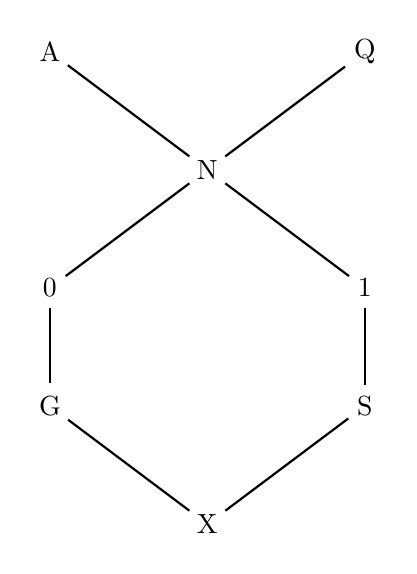
\begin{tikzpicture}
		\GraphInit[vstyle=Empty]
		\Vertex{A}
		\Vertex[x=4,y=0]{Q}
		\Vertex[x=2,y=-1.5]{N}
		\Vertex[x=0,y=-3]{0}
		\Vertex[x=4,y=-3]{1}
		\Vertex[x=0,y=-4.5]{G}
		\Vertex[x=4,y=-4.5]{S}
		\Vertex[x=2,y=-6]{X}
		\Edges(A,N,Q) 
		\Edges(0,N,1)
		\Edges(0,G)
		\Edges(1,S)
		\Edges(G,X,S)
		\end{tikzpicture}
		
		Where symbols on a graph mean:
		\begin{itemize}
			\item $A = (\alpha_{i1}, \alpha_{i2}, \ldots, \alpha_{iK} )^{'}$
			\item $Q = (q_{j1}, q_{j2}, \ldots, q_{jK} )^{'}$
			\item $N = \eta_{ij} = 1- \prod\limits_{k=1}^{K} \left( 1 - \alpha_{ik} \right)^{q_{jk}}$
			\item $G = g_j$
			\item $S = 1-s_j$
			\item $X = X_{ij}$
			\item $P(X_{ij} = 1 | \eta_{ij}) = (1-s_j)^{\eta_{ij}} \cdot g_j^{1-\eta_{ij}}$
		\end{itemize}
	\end{multicols} 
	\caption{A graphical representation of the \textit{i}-th examinee response process to item \textit{j} in~the~DINO model \cite{de_la_torre_2009}.}\label{graph_dino}
\end{figure}

\section{The NIDA model}

The noisy inputs, deterministic, ``and'' gate model (NIDA) was discussed in 1999 by Maris \cite{nida_maris} and described in detail by Junker and Sijtsma in 2001 \cite{nida_model}. Like DINA, the NIDA model belongs to the non-compensatory type of models, and the same as the DINA model it is an example of models with a conjunctive condensation rule (all required attributes need to be present). The difference between those two models is that in the DINA model there is no matter which skill or skills are missing -- probability for a correct response to an item is the same, NIDA model distinguishes these cases and probability differs depending on missing attributes. 

For the NIDA model are needed variables $X_ij$, $\alpha_{ik}$, and $q_{jk}$ which were described earlier and the latent variable $\zeta_{ijk} \in \{0,1\}$ which is defined, indicating whether examinee $i$ correctly apply an attribute $k$ for the item $j$ (examinee's performance in the context of an~item is compatible with possessing skill $\zeta_{ijk}=1$ or not $\zeta_{ijk}=0$) \cite{book_tables}. This, in turn, is~related to the definition of slipping and guessing parameters.

Already known DINA and DINO models both model slipping and guessing processes at the item level. In the NIDA model, in contrast to DINA and DINO, guessing and slipping occur at the skill rather than item level. To summarize, the latent variables $\zeta_{ijk}$ are related to the examinee's skill profiles $\alpha_{i}$ according to the probabilities

\begin{equation}
s_k = P(\zeta_{ijk} = 0 | \alpha_{ik} = 1, q_{jk} = 1),
\end{equation}
\begin{equation}
g_k = P(\zeta_{ijk} = 1 | \alpha_{ik} = 0, q_{jk} = 1),
\end{equation}
and, what is important,
\begin{equation}
P(\zeta_{ijk} = 1 | \alpha_{ik} = \alpha, q_{jk} = 0) \equiv 1,
\end{equation}
no matter what is the value of $\alpha_{ik}$ (can take any value $\alpha \in \{0,1\}$). The observed response to the item $j$ by examinee $i$ is expressed through
\begin{equation}
X_{ij} = \prod\limits_{k: q_{jk}=1} \zeta_{ijk} = \prod\limits_{k=1}^{K} \zeta_{ijk}.
\end{equation}

\noindent While the slipping $s_k$ and guessing $g_k$ parameters (probabilities of correctly applying each of the measured skills) are determined and while the skill profile $\alpha_{i}$ and the weight matrix $Q_{J\times K}$ are known, the correct response probability in~the~NIDA model (the probability of correctly applying measured skills for the item) can be computed. The correct response probability for a single item is expressed through 
\begin{equation}
P(X_{ij} = 1 | \alpha_i, g, s) = \prod\limits_{k=1}^{K} P(\zeta_{ijk} = 1 | \alpha_{ik}, q_{jk}) = \prod\limits_{k=1}^{K} \left[ (1-s_k)^{\alpha_{ik}} \cdot g_k^{(1-\alpha_{ik})} \right] ^{q_{jk}}.
\end{equation}

The NIDA model has restrictive assumptions -- constraints of equality across the items. This means that the model provides one slipping ($s_k$) and one guessing ($g_k$) parameter per skill, but the values of slipping and guessing parameters have to be the same across the items. The number of model parameters is not influenced by the number of items, it~increases with the number of skills. 

An extension of the NIDA model is the generalized noisy inputs, deterministic, ``and'' gate (G-NIDA) model where the slipping and guessing parameters are permitted to differ also across the items. It is going to be described in the next section. 

\section{The G-NIDA model}

The generalized noisy inputs, deterministic, ``and'' gate (G-NIDA) model, as it was mentioned before, is an extension of the NIDA model. In the G-NIDA model slipping and guessing parameters are allowed to vary not only across the attributes but also across the items
\begin{equation}
s_{jk} = P(\zeta_{ijk} = 0 | \alpha_{ik} = 1, q_{jk} = 1),
\end{equation}
\begin{equation}
g_{jk} = P(\zeta_{ijk} = 1 | \alpha_{ik} = 0, q_{jk} = 1).
\end{equation}

\noindent This property leads to the correct response probability in the G-NIDA model in the form
\begin{equation}
P(X_{ij} = 1 | \alpha_i, g_j, s_j) = \prod\limits_{k=1}^{K} \left[ (1-s_{jk})^{\alpha_{ik}} \cdot g_{jk}^{(1-\alpha_{ik})} \right] ^{q_{jk}},
\end{equation}
where the terms above are the same as described in the description of the NIDA model.
 
\section{Methodology}

In this Section are described the procedure and the methods used to carry out the simulations and test their quality: the Joint Maximum Likelihood Estimation, which was used for fitting Cognitive Diagnosis Models (CDMs), and the statistics and measures necessary to evaluate these fits: log-likelihood value, Akaike and Bayesian Information Criteria and measures based on confusion matrix (accuracy, informedness, markedness, and their geometric mean).

\subsection{Joint Maximum Likelihood Estimation}

The Joint maximum likelihood estimation (JMLE) is a parameteric approach to fit a Cognitive Diagnosis Models to the response data an estimate both the item parameters and examinee attribute profiles\footnote{Source: https://cran.r-project.org/web/packages/NPCD/NPCD.pdf (access: VIII 2020)}. Joint Maximum Likelihood Estimation procedure involves maximizing the overall likelihood function by means of the parameter estimates obtained by the separate MLE procedures for the items and examinees. The intent is to obtain a global maximum for the overall likelihood function. 

As is known from Section \ref{section:term_notation}, $I$ examinees possess their skill profiles and each of these examinees responds to the $J$ items of the test. The responses are dichotomously scored, $x_{ij} \in \{0,1\}$, where $i$ $(i = 1, 2, \ldots, I)$ indicates the examinee and $j$ $( j = 1, 2, \ldots, J)$ defines the item. 
For each examinee there is a vector of item responses of length $J$ denoted by $(x_{i1}, x_{i2}, \ldots, x_{iJ} | \theta_i)$, where $\theta_i$ is $K$-dimensional latent vector (the examinee's skill profile). Under the local independence assumption (a standard assumption for item factor analysis), the $x_{ij}$ are statistically independent for all examinees having the same skill profile. The resulting $I \times J$ matrix of item responses (the response matrix) is already known as $X$. If $\Theta$ is the vector of all examinees' skill profiles $(\theta_1, \theta_1, \ldots, \theta_I)$, the probability of $X$ is given by the joint likelihood function specified \cite{jmle} as

\begin{equation}
	\mathcal{L}(\Theta|X) = P(X|\Theta) = \prod_{i=1}^{I} \prod_{j=1}^{J} P_j (\theta_i)^{x_{ij}} Q_j(\theta_i)^{1-x_{ij}},
\end{equation}

\noindent where $Q_j = 1 - P_j$. As typically, it is the natural logarithm of the likelihood function that one maximizes. So, the function being maximized is given by

\begin{equation}
	l(\Theta|X) = \log\: \mathcal{L}(\Theta|X) = \sum_{i=1}^{I} \sum_{j=1}^{J} \left[ x_{ij}\; \log\: P_j(\theta_i) + (1-x_{ij})\; \log\:  Q_j(\theta_i) \right] + const.
\end{equation}

\noindent Thus, the Joint Maximum Likelihood Estimator is defined \cite{jmle2} as

\begin{equation}
	\hat{\Theta} = \underset{\Theta}{\arg\max} \log\: \mathcal{L}(\Theta|X). 
\end{equation}

\texttt{JMLE()} function in \texttt{NPCD} library returns Joint Maximum Likelihood Estimates of item parameters and examinees skill profiles in CDMs. The algorithm starts from the nonparametric estimation of skill profiles for both the conjunctive and disjunctive CDMs, implemented by the \texttt{AlphaNP()} function. Algorithms choose the skill profile with the smallest loss function value. When the attribute profiles are chosen, then the \texttt{JMLE()} function iteratively estimates item parameters and skill profiles using MLE until the algorithm converges\footnote{Source: https://cran.r-project.org/web/packages/NPCD/NPCD.pdf (access: VIII 2020)}.

\subsection{Log-likelihood value}

Log-likelihood value is a measure of goodness of fit for any model. Log-likelihood can take values between $-\infty$ to $+\infty$. Higher the value of log-likelihood, better is the fit of the model. Log-likelihood value belongs to relative fit evaluation type because it is a~function of sample size, which means that it cannot be used alone as an index of fit and the absolute look at the value cannot give any indication but it can be used to compare the fit between different models\footnote{Source: https://medium.com/@analyttica/log-likelihood-analyttica-function-series-cb059e0d379 (access: VIII 2020)}. 

\subsection{AIC and BIC criteria}

Akaike and Bayesian information criteria are the two most commonly used criteria in model
selection and they are both penalized-likelihood criteria. They are goodness-of-fit tests to assess the
performance of a model with respect to how well it explains the data. A lower AIC or BIC value indicates a better fit \cite{aic_bic}.

\subsubsection{Akaike information criterion}

Akaike information criterion was proposed by Akaike in 1974 \cite{aic}. The formula for AIC is as follows

\begin{equation}
	AIC = -2 \log{\mathcal{L}(\hat{\Theta})} + 2k,
\end{equation}

\noindent where $\Theta$ is the vector of model parameters, $\mathcal{L}(\hat{\Theta})$ is the value of the likelihood function and $k$ is the number of estimated parameters. 

The first element is the value of the likelihood function, which is the probability of obtaining the data given the candidate model, multiplied by $-2$. Ignoring the second element, the model with the~minimum AIC is the best one. However, to the first component is added the number of estimated parameters multiplied by 2. The more parameters, the higher the value of the AIC, which means that the model is penalized for its complexity. As a~result, it has to be considered whether a better fit by creating a more complex model is worth the penalty imposed by requiring more parameters.

\subsubsection{Bayesian information criterion}

Bayesian information criterion was proposed by Schwarz in 1978 \cite{bic}. It is another model selection criterion based on information theory and it is closely related to the Akaike information criterion. The formula for BIC is as follows

\begin{equation}
	BIC = -2 \log{\mathcal{L}(\hat{\Theta})} + k\log{n},
\end{equation}

\noindent where $\Theta$ is the vector of model parameters, $\mathcal{L}(\hat{\Theta})$ is the value of the likelihood, $k$ is the number of estimated parameters and $n$ is the number of observations (sample size). 

The difference between the AIC and the BIC is the penalty imposed for the number of parameters, it is larger in BIC than in AIC. The penalty in BIC resolves the problem of overfitting, which is possible in AIC because of increasing the likelihood by adding parameters.

\subsection{Confusion matrix}

Contingency Table is an $N \times N$ matrix, where columns correspond to the correct decision classes and rows correspond to decisions predicted by the classifier. The number $n_{ij}$ at the intersection of row $i$ and column $j$ is the number of examples from the $j$-th class that were classified to the $i$-th class. Special attention is given to $2 \times 2$ tables, which are called confusion matrices. All possible results in the binary classification are:

\begin{itemize}
	\item True Positive -- the observation was positive and was classified as positive,
	\item False Positive -- the observation was negative and was classified as positive,
	\item False Negative -- the observation was positive and was classified as negative,
	\item True Negative -- the observation was negative and was classified as negative,
\end{itemize}

\noindent and they are presented in Table \ref{tab:confusion_matrix}.

\begin{table}[H]
	\centering
	\begin{tabular}{c c | c | c} 
		 & & \multicolumn{2}{c}{Actual class} \\
		 & & Positive & Negative \\
		 \hline
		 {\rule{0pt}{3ex}} \multirow{2}{*}{Predicted class} & Positive & True Positive (TP) & False Positive (FP) \\\cmidrule{2-4}
		 & Negative & False Negative (FN) & True Negative (TN)  \\
	\end{tabular}
	\caption{The confusion matrix.}
	\label{tab:confusion_matrix} 
\end{table}

The definitions of all measures come from the work of D. Powers \cite{powers2011evaluation}, but before defining mentioned earlier accuracy, informedness and markedness, it is worth to know the basic measures:

\begin{itemize}
	\item Sensitivity (also called Recall or True Positive Rate) is the ratio of correctly classified positive cases to all observations, which are really positive. It measures the percentage of positive cases found by the model. The formula of sensitivity is as follows
	$$ TPR = \frac{TP}{TP + FN}. $$
	\item Specificity (also called Inverse Recall or True Negative Rate) is the ratio of correctly classified negative cases to all observations, which are really negative. It measures the percentage of negative cases found by the model. The formula of specificity is as follows
	$$ TNR = \frac{TN}{TN + FP}. $$
	\item Precision (also called Confidence or True Positive Accuracy) is the ratio of correctly classified positive cases to all observations classified as positive. It measures the percentage of samples which were correctly classified as positive. The formula of precision is as follows
	$$ TPA = \frac{TP}{TP + FP}. $$
	\item Inverse Precision (also called True Negative Accuracy) is the ratio of correctly classified negative cases to all observations classified as negative. It measures the percentage of samples which were correctly classified as negative. The formula of inverse precision is as follows
	$$ TNA = \frac{TN}{TN + FN}. $$
\end{itemize}

\subsubsection{Accuracy}

The accuracy combines sensitivity and specificity. It measures the ratio of correctly classified cases to the number of all observations. It takes into account both positive and negative observations. For this reason, it copes very well, when observations from both classes are significant for the researcher. That is why this measure is used to evaluate the fit of the models -- it allows seeing the percentage of well-classified by the model skills. The formula of accuracy is as follows

$$ ACC = \frac{TP + TN}{TP + TN + FP + FN}. $$

\subsubsection{Informedness}

``Informedness quantifies how informed a predictor is for the specified condition, and specifies the probability that a prediction is informed in relation to the condition (versus chance)'' \cite{powers2011evaluation}. In other words, informedness determines how well-informed the test is about positives and negatives with respect to randomness. Informedness considers both real positives and real negatives cases. For the binary case, there is a relation Informedness = Sensitivity + Specificity – 1. The formula of informedness is as follows

$$ \text{Informedness} = \frac{TP}{TP + FN}  +  \frac{TN}{TN + FP} - 1 = \frac{TP}{TP + FN} - \frac{FP}{TN + FP}. $$
	
\subsubsection{Markedness}

``Markedness quantifies how marked a condition is for the specified predictor and specifies the probability that a condition is marked by the predictor (versus chance)'' \cite{powers2011evaluation}. This means that markedness determines how well the population is being tested against randomness, measures trustworthiness of positive and negative predictions by the test. Markedness considers both predicted positives and predicted negatives cases. For the binary case, there is a relation Markedness = Precision + Inverse Precision – 1. The formula of markedness is as follows

$$ \text{Markedness} = \frac{TP}{TP + FP} + \frac{TN}{TN + FN} - 1 = \frac{TP}{TP + FP} - \frac{FN}{TN + FN}. $$

\subsubsection{The Matthews Correlation}

``The Matthews correlation is a contingency matrix method of calculating the Pearson product-moment correlation coefficient'' \cite{powers2011evaluation}. This is the geometric mean of informedness and markedness and it describes how much the method results (predictions) correlate with the real cases. This means that it is a clear indication of how well the method is performing and its formula is as follows

$$ COR = \text{sign}(I)\ \sqrt{IM} = \text{sign}(M)\ \sqrt{IM}. $$


\chapter{Simulations}\label{chapter:simulations}

In this chapter, the analysis of the Cognitive Diagnosis Models will be carried out. There are different reasons for the occurrence of model–data misfit in cognitive diagnosis modelling.  The~analysis will consist of examining two causes of a misfit: CDM and $Q$-matrix misspecifications,  because both the CDM and the $Q$-matrix are integral parts of the modelling process, both misspecifications can be easily investigated, can significantly affect classification accuracy and can even interact causing the estimation process to be worse. The first part will concern the CDM misspecification and comparison of the models' robustness, the second one will be conducted, to measure the effect of $Q$-matrix misspecification. 

The simulations were carried out in the \texttt{R} environment, which contains extensive and powerful tools for Cognitive Diagnosis Models analysis. Self-made functions were used to create random skill profiles, random $Q$-matrix, and as a consequence to simulate the models -- the result of this function is the response data. The code is available in Appendix \ref{appendix}. \texttt{CDM} (Cognitive Diagnosis Modeling) and \texttt{NPCD} (Nonparametric Methods for Cognitive Diagnosis) libraries were used for model estimation. Especially, \texttt{JMLE()} (Joint Maximum Likelihood Estimation Of Item Parameters And Examinee Attribute Profiles) function was used in the CDM misspecification (Section \ref{section:cdm_misspec}) and \texttt{gdina()} function was used for estimating the DINA model in the $Q$-matrix misspecification (Section \ref{section:qmat_misspec}).

\section{CDM misspecification}\label{section:cdm_misspec}

Four different models, described in the previous chapter, were selected for comparison: DINA, DINO, NIDA, and G-NIDA. These models were chosen because they can be estimated using the same methods (\texttt{JMLE()} function) and they are all defined using the same parameters: slipping and guessing one. In the DINA and DINO models slipping and guessing parameters occur at the item level, in the NIDA model, those parameters occur at the attribute level and in the G-NIDA model, those parameters these parameters apply to both item and attribute levels. 

For each of mentioned models, the response data was generated. The sample size, number of items, and number of skills were fixed to $I=5000$, $J=30$, and $K=5$, respectively. The sample size corresponds to the number of randomly generated skill patterns (one for each of the examinees) selected from the skill class consisting of all possible profiles ($2^K = 2^5 = 32$). The test was composed of three item types: requiring one, two, or three skills, and each of these types occurred the same number of times (each skill is required in the test exactly 10 times), as shown by the $Q$-matrix \ref{tab:qmatrix_sim}. For the DINA, DINO, and NIDA models, the slipping and guessing parameters were set to $0.20$, for the G-DINA model, $s$ and $g$ parameters were randomly generated with a uniform distribution and could take a value from the set $\{0.1,0.2,0.3\}$. 

\begin{table}[H]
	\centering
	\begin{tabular}{c c c c c c} 
		\hline
		{\rule{0pt}{3ex}} & \multicolumn{5}{l}{Skill} \\
		Item & $\alpha_1$ & $\alpha_2$ & $\alpha_3$ &  $\alpha_4$ & $\alpha_5$ \\ [0.5ex] 
		\hline
		1 & 1 & 0 & 0 & 0 & 0 \\ 
		2 & 0 & 1 & 0 & 0 & 0 \\
		3 & 0 & 0 & 1 & 0 & 0 \\
		4 & 0 & 0 & 0 & 1 & 0 \\
		5 & 0 & 0 & 0 & 0 & 1 \\
		6 & 1 & 0 & 0 & 0 & 0 \\ 
		7 & 0 & 1 & 0 & 0 & 0 \\
		8 & 0 & 0 & 1 & 0 & 0 \\
		9 & 0 & 0 & 0 & 1 & 0 \\
		10 & 0 & 0 & 0 & 0 & 1 \\ 
		11 & 1 & 1 & 0 & 0 & 0 \\ 
		12 & 1 & 0 & 1 & 0 & 0 \\
		13 & 1 & 0 & 0 & 1 & 0 \\
		14 & 1 & 0 & 0 & 0 & 1 \\
		15 & 0 & 1 & 1 & 0 & 0 \\
		16 & 0 & 1 & 0 & 1 & 0 \\  
		17 & 0 & 1 & 0 & 0 & 1 \\ 
		18 & 0 & 0 & 1 & 1 & 0 \\
		19 & 0 & 0 & 1 & 0 & 1 \\
		20 & 0 & 0 & 0 & 1 & 1 \\ 
		21 & 1 & 1 & 1 & 0 & 0 \\
		22 & 1 & 1 & 0 & 1 & 0 \\ 
		23 & 1 & 1 & 0 & 0 & 1 \\ 
		24 & 1 & 0 & 1 & 1 & 0 \\
		25 & 1 & 0 & 1 & 0 & 1 \\ 
		26 & 1 & 0 & 0 & 1 & 1 \\ 
		27 & 0 & 1 & 1 & 1 & 0 \\ 
		28 & 0 & 1 & 1 & 0 & 1 \\ 
		29 & 0 & 1 & 0 & 1 & 1 \\ 
		30 & 0 & 0 & 1 & 1 & 1\\ [1ex] 
		\hline
	\end{tabular}
	\caption{The weight matrix $Q_{30 \times 5}$ used for comparison of CDMs.}
	\label{tab:qmatrix_sim} 
\end{table}

The analysis consists of two parts -- two types of fit evaluation. The statistics from the first part were used for a relative fit evaluation which concerns the process of selecting the best-fitting model from a set of competing models. Theoretically, the results of the fit statistics should be the best for the true model. The second part is an absolute fit evaluation, which concerns the process of determining whether the model is a good fit for the data. Theoretically, fit statistics should reject misspecified models, practically it is likely that more than one model will be a good fit to the data due to the fact that the models share common characteristics. 

The first component is based on examining the final overall log-likelihood values from the estimated item parameters and attribute profiles based on the specified model, the overall AIC and BIC statistics for outputs generated by estimation function (\texttt{JMLE()}). The second component verifies the goodness of the skills classification (how many of the examinees have well classified skills), the probability that the skill will be well identified and the values of the informedness, markedness parameters, as well as their geometrical mean. 

\subsection{Results}

The first component concerns a relative fit evaluation for CDM misspecification. In~Table \ref{tab:estimations} and in Figure \ref{heatmap_stats} are presented results of examining log-likelihood values, AIC statistics and BIC statistics. The best results (the highest log-likelihood value and the lowest AIC and BIC values) are expected for the true models. 

For the true G-NIDA model, the value of BIC statistics is lower for estimated NIDA model. Possible reason is high penalty imposed for the number of parameters -- simpler NIDA model has lower penalty, so it obtains better results. For the true NIDA model, log-likelihood value is higher for estimated G-NIDA model. This situation also has easy explanation -- log-likelihood does not include the penalty, so richer model will always be chosen. It is necessary to remember that those models are only slightly different and the difference almost always is their complexity. Other statistics for NIDA and G-NIDA models are very similar too, but true models obtain better results. For other cases, especially for all cases for the AIC statistics, the true models always obtain the best results. This means that AIC statistics is the best for comparing Cognitive Diagnosis Models -- it has penalty, so it would not choose just the most complex model, but the value of penalty is not too high, so it would not choose the easiest one. 

Interestingly, the comparison of the statistics' results for true NIDA and G-NIDA models and estimated DINA model are also quite satisfying, the results for DINA do not differ much from those obtained for the true models. The opposite situation is the same, especially for G-NIDA model. The G-NIDA model is a good fit for the response data simulated with DINA and NIDA models. This is understandable because G-NIDA is a saturated model and saturated models fit the data better than reduced CDMs because of their more complex parameterization. However, saturated CDMs require larger sample sizes to be estimated precisely, reduced CDMs are simpler. 

Considering the results obtained for the DINO as an estimated model, it can be seen that it has the worst results for the data simulated with DINA, NIDA and especially with G-NIDA model. Worth the attention is also the case with DINO as a true model. The best results are obtained for the DINO itself, which is not a surprise but the worst results are obtained for an estimated G-NIDA model and for the NIDA model, they are also quite bad. The possible reason for this situation is~a belonging to other groups. DINA, NIDA and G-NIDA models are non-compensatory, while the DINO model belongs to the group of compensatory models. The most similar statistics values to the values for the true DINO model has the DINA model and it could be caused by the similar structures of DINA and DINO models. 

The analysis of the obtained log-likelihood, AIC and BIC values, presented in Table \ref{tab:estimations} and in Figure \ref{heatmap_stats} with the use of heatmaps, gave interesting results. Considering the robustness for the model misspecification, the conclusion is that for chosen competing models (DINA, DINO, NIDA and G-NIDA) the most optimal one is DINA model.

\begin{table}[H]
	\centering
	\begin{tabular}{l l c c c c} 
		\hline
		{\rule{0pt}{3ex}} \multirow{2}{*}{True model} & \multirow{2}{*}{Statistics} & \multicolumn{4}{c}{Estimated models} \\\cmidrule{3-6}
		& & DINA & DINO & NIDA & G-NIDA \\ [0.5ex]
		\hline 
		{\rule{0pt}{3ex}} \multirow{3}{*}{DINA model} & log-likelihood & \textbf{-72190.15} & -82112.43 & -76655.75 & -73968.53 \\ 
		& AIC & \textbf{144562.3} & 164406.9 & 153393.5 & 148599.1 \\ 
		& BIC & \textbf{145155.4} & 164999.9 & 153660.7 & 150756.2\\ 
		[0.5ex] 
		\hline
		{\rule{0pt}{3ex}} \multirow{3}{*}{DINO model} & log-likelihood & -82081.78 & \textbf{-72241.84} & -119062.16 & -182399.53 \\ 
		& AIC & 164345.6 & \textbf{144665.7} & 238206.3 & 365461.1 \\ 
		& BIC & 164938.6 & \textbf{145258.8} & 238473.5 & 367618.3\\ 
		[0.5ex] 
		\hline
		{\rule{0pt}{3ex}} \multirow{3}{*}{NIDA model} & log-likelihood & -59309.23 & -67473.71 & -58128.59 & \textbf{-58122.48} \\ 
		& AIC & 118800.5 & 135129.4 & \textbf{116339.2} & 116907.0 \\ 
		& BIC & 119393.5 & 135722.5 & \textbf{116606.4} & 119064.2\\ 
		[0.5ex] 
		\hline
		{\rule{0pt}{3ex}} \multirow{3}{*}{G-NIDA model} & log-likelihood & -57047.97 & -66877.56 & -56474.90 & \textbf{-55316.41} \\ 
		& AIC & 114277.9 & 133937.1 & 113031.8 & \textbf{111294.8} \\ 
		& BIC & 114871.0 & 134530.2 & \textbf{113299.0} & 113452.0\\ 
		[0.5ex] 
		\hline
	\end{tabular}
	\caption{Values of statistics for scoring the correctness of fitting different models to the~specified model.}
	\label{tab:estimations} 
\end{table}

\begin{figure}[h!]
	\centering
	\includegraphics[width=0.7\textwidth]{Heatmaps_relative_fit.png}
	\caption{Heatmaps for log-likelihood, AIC and BIC statistics.}
	\label{heatmap_stats}
\end{figure}

The first part of the second component is examination how many skill profiles of the examinees were estimated correctly, how many profiles had four, three, two, one or none of the five skills identified correctly. The model is good when it classifies most of the skills correctly. Figures \ref{comparison_dina}, \ref{comparison_dino}, \ref{comparison_nida} and \ref{comparison_gnida} show the number of examinees with an amount of well-classified skills for the DINA, DINO, NIDA, G-NIDA models as a true model respectively. In the upper left corner of each barplot there is a weighted mean value that allows assessing how many skills on average are correctly determined by the model. In each case, the number of all skills classified correctly was the highest for true models and the percentage was between 64\% and 72\%. Next conclusions are also similar as in the previous case. DINA, NIDA and G-NIDA models are good fits for each other (when the model used for simulation is one of them), the difference in the weighted means is not greater than 0.1. When the response data obtained from the DINA model were estimated by DINO model and when for the true DINO model the data were estimated by DINA model, only around 15\% of skill profiles were classified fully correct. The results when the true model was DINO, for NIDA and G-NIDA models estimation were even worse and amounted to less than 6\%. None of the estimated models (except the true DINO model) classified on average more than 3.8 skills.

\begin{figure}[h!]
	\centering
	\includegraphics[width=\textwidth]{DINA_skills_classification_col.png}
	\caption{Comparison of results for the DINA model simulated.}
	\label{comparison_dina}
\end{figure}

\begin{figure}[h!]
	\centering
	\includegraphics[width=\textwidth]{DINO_skills_classification_col.png}
	\caption{Comparison of results for the DINO model simulated.}
	\label{comparison_dino}
\end{figure}

\begin{figure}[h!]
	\centering
	\includegraphics[width=\textwidth]{NIDA_skills_classification_col.png}
	\caption{Comparison of results for the NIDA model simulated.}
	\label{comparison_nida}
\end{figure}

\begin{figure}[h!]
	\centering
	\includegraphics[width=\textwidth]{GNIDA_skills_classification_col.png}
	\caption{Comparison of results for the G-NIDA model simulated.}
	\label{comparison_gnida}
\end{figure}

The second part of the second component was examining the accuracy of the estimated models -- how often skills are well defined. Accuracies for each skill and for whole response data were obtained and the results are presented in Table \ref{tab:estimation_skills}. Comparison of results for individual skills does not give any special conclusions, there is no pattern corresponding to the specific skill nor model. This means that models check all of the skills at a similar level. If the $Q$-matrix is well-created, there should be no dependencies of results for individual skills on estimation. Accuracies calculated for models, in general, are presented in the last column. There is no surprise that for the true model the skills are more often well defined. The results for all of the models confirm the conclusions received in the previous part.

\begin{table}[H]
	\centering
	\begin{tabular}{l c c c c c c} 
		\hline
		{\rule{0pt}{3ex}} & \multicolumn{6}{c}{DINA model} \\ 
		& $\alpha_1$ & $\alpha_2$ & $\alpha_3$ & $\alpha_4$ & $\alpha_5$ & \textbf{mean} \\ [0.5ex]
		\hline 
		{\rule{0pt}{3ex}}DINA & 0.9098 & 0.9090 & 0.9216 & 0.9116 & 0.9116 & \textbf{0.91272} \\ 
		DINO & 0.7522 & 0.7680 & 0.7316 & 0.7764 & 0.7504 & \textbf{0.75572} \\
		NIDA & 0.8948 & 0.9010 & 0.9030 & 0.8908 & 0.8944 & \textbf{0.89680} \\
		G-NIDA & 0.8958 & 0.9058 & 0.9048 & 0.8930 & 0.8952 & \textbf{ 0.89892} \\ [0.5ex] 
		\hline
		{\rule{0pt}{3ex}} & \multicolumn{6}{c}{DINO model} \\ 
		& $\alpha_1$ & $\alpha_2$ & $\alpha_3$ & $\alpha_4$ & $\alpha_5$ & \textbf{mean} \\ [0.5ex]
		\hline 
		{\rule{0pt}{3ex}}DINA & 0.7358 & 0.7722 & 0.7522 & 0.7588 & 0.7496 & \textbf{0.75372} \\ 
		DINO & 0.9054 & 0.9034 & 0.9080 & 0.9072 & 0.9140 & \textbf{0.90760} \\
		NIDA & 0.5084 & 0.5180 & 0.5284 & 0.5158 & 0.5156 & \textbf{0.51724} \\
		G-NIDA & 0.6076 & 0.6814 & 0.5664 & 0.6218 & 0.7474 & \textbf{ 0.64492} \\ [0.5ex] 
		\hline
		{\rule{0pt}{3ex}} & \multicolumn{6}{c}{NIDA model} \\ 
		& $\alpha_1$ & $\alpha_2$ & $\alpha_3$ & $\alpha_4$ & $\alpha_5$ & \textbf{mean} \\ [0.5ex]
		\hline 
		{\rule{0pt}{3ex}}DINA & 0.8914 & 0.8908 & 0.8908 & 0.8870 & 0.8876 & \textbf{0.88952} \\ 
		DINO & 0.7446 & 0.7276 & 0.7120 & 0.7130 & 0.7132 & \textbf{0.72208} \\
		NIDA & 0.9098 & 0.9154 & 0.9072 & 0.9032 & 0.9128 & \textbf{0.90968} \\
		G-NIDA & 0.9078 & 0.9144 & 0.9070 & 0.9038 & 0.9104 & \textbf{ 0.90868} \\ [0.5ex] 
		\hline
		{\rule{0pt}{3ex}} & \multicolumn{6}{c}{G-NIDA model} \\ 
		& $\alpha_1$ & $\alpha_2$ & $\alpha_3$ & $\alpha_4$ & $\alpha_5$ & \textbf{mean} \\ [0.5ex]
		\hline 
		{\rule{0pt}{3ex}}DINA & 0.9108 & 0.9106 & 0.9272 & 0.9248 & 0.9316 & \textbf{0.92100} \\ 
		DINO & 0.7496 & 0.7148 & 0.7262 & 0.7544 & 0.7364 & \textbf{0.73628} \\
		NIDA & 0.9180 & 0.9186 & 0.9378 & 0.9380 & 0.9334 & \textbf{0.92916} \\
		G-NIDA & 0.9206 & 0.9240 & 0.9398 & 0.9402 & 0.9404 & \textbf{ 0.93300} \\ [0.5ex] 
		\hline
	\end{tabular}
	\caption{Mean values of skills classification for each model.}
	\label{tab:estimation_skills} 
\end{table}

The last part of the second component concerning an absolute fit evaluation for CDM misspecification is examining informedness (which determines how well-informed the test is relative to randomness), markedness (which determines how well the population is tested against randomness) and their geometric mean -- correlation (which describes how much the results of the method are correlated with the actual assessment). The results are presented in Table \ref{tab:confusion_values} and in Figure \ref{heatmap_measures}, which includes the heatmaps for each measure. The values obtained for these measures are more diverse than previously. For example, the values of the informedness for the NIDA model, when the true model was DINO, is very low -- less than 3\%, which results in the correlation, between the estimation and real response data, equal to about 12\%. However, all of the results confirm previous conclusions -- measures have the highest values for the true models, have similar results for all of the non-compensatory models and have the worst values for NIDA and G-NIDA models, when the true model is DINO.

\begin{table}[H]
	\centering
	\begin{tabular}{l l c c c c} 
		\hline
		{\rule{0pt}{3ex}} \multirow{2}{*}{True model} & \multirow{2}{*}{Measure} & \multicolumn{4}{c}{Estimated models} \\\cmidrule{3-6}
		& & DINA & DINO & NIDA & G-NIDA \\ [0.5ex]
		\hline 
		{\rule{0pt}{3ex}} \multirow{3}{*}{DINA model} & informedness & \textbf{0.8253833} & 0.5140384 & 0.7936219 & 0.7978157 \\ 
		& markedness & \textbf{0.8255185} & 0.6198476 & 0.7935927 & 0.7978475 \\ 
		& correlation & \textbf{0.8254509} & 0.5644692 & 0.7936073 & 0.7978316\\ 
		[0.5ex] 
		\hline
		{\rule{0pt}{3ex}} \multirow{3}{*}{DINO model} & informedness & 0.5048264 & \textbf{0.8152497} & 0.0284173 & 0.2858251 \\ 
		& markedness & 0.6141829 & \textbf{0.8152247} & 0.5103258 & 0.4896448 \\ 
		& correlation & 0.5568265 & \textbf{0.8152372} & 0.1204246 & 0.3741026\\ 
		[0.5ex] 
		\hline
		{\rule{0pt}{3ex}} \multirow{3}{*}{NIDA model} & informedness & 0.7795057 & 0.4474721 & \textbf{0.8195347} & 0.8175810 \\ 
		& markedness & 0.7832871 & 0.6204171 & \textbf{0.8199320} & 0.8183015 \\ 
		& correlation & 0.7813941 & 0.5268960 & \textbf{0.8197333} & 0.8179412\\ 
		[0.5ex] 
		\hline
		{\rule{0pt}{3ex}} \multirow{3}{*}{G-NIDA model} & informedness & 0.8421491 & 0.4757360 & 0.8585197 & \textbf{0.8662798} \\ 
		& markedness & 0.8424090 & 0.6394361 & 0.8590959 & \textbf{0.8675957} \\ 
		& correlation & 0.8422790 & 0.5515458 & 0.8588077 & \textbf{0.8669375}\\ 
		[0.5ex] 
		\hline
	\end{tabular}
	\caption{Values of measures for different models.}
	\label{tab:confusion_values} 
\end{table}

\begin{figure}[h!]
	\centering
	\includegraphics[width=0.7\textwidth]{Heatmaps_absolute_fit.png}
	\caption{Heatmaps for informedness, markedness and correlation measures.}
	\label{heatmap_measures}
\end{figure}

Summarizing, after comparing the results of the estimation with the results for the simulation using the true model, all of the statistics and measures returned the best values for the true model. Obtained results mean that all of the models were good enough to fit the data correctly. Estimating the response data with the use of the DINO model for DINA, NIDA and G-NIDA as a true model, gave the worst results. The possible reason for this situation is the type of the group to which this model belongs -- the DINO is an example of the compensatory model, while the other three belong to the non-compensatory group. G-NIDA is a saturated model -- is more general, so theoretically and practically it is a good fit for other models from the same group (DINA and NIDA models). However, it requires more complex computations. The DINA model, which is much easier than G-NIDA, also obtained very good results and it is the best fit for the DINO model (which is in a group of non-compensatory models) that is why it is going to be used in Section \ref{section:qmat_misspec}.
  


\section{Q-matrix misspecification}\label{section:qmat_misspec}

\subsection{Results}

\chapter{Analysis of the real data}\label{chapter:real_data}

{\backmatter \chapter{Summary and discussion}}

\appendix
{\chapter{Functions}}\label{appendix}

\noindent The appendix lists the functions that were used to run the simulations -- generating a~random $Q$-matrix, random skill profiles and, as a~result, a response matrix. \vspace{5pt}


\begin{itemize}

\item  Function \texttt{solve\_test()} is a solution of the test, what means it returns the response data -- binary matrix with value 1 if examinee solved the item correctly or 0 if not. The possible Cognitive Diagnosis Models are DINA, DINO, NIDA and G-NIDA.
\begin{verbatim}
solve_test <- function(sk_prof, Q_matrix, model, s, g){
good_ans_prob <- matrix(0,dim(Q_matrix)[1],1)
result <- matrix(0,dim(Q_matrix)[1],1)
if(model == "DINA")
{
for(i in 1:nrow(Q_matrix)){
Q_vec <- Q_matrix[i,]
eta <- prod(sk_prof^Q_vec)
good_ans_prob[i] <- (1-s[i])^eta * g[i]^(1-eta)
result[i] <- rbinom(1, 1, good_ans_prob[i])
}
}
if(model == "DINO")
{
for(i in 1:nrow(Q_matrix)){
Q_vec <- Q_matrix[i,]
eta <- 1 - prod((1-sk_prof)^Q_vec)
good_ans_prob[i] <- (1-s[i])^eta * g[i]^(1-eta)
result[i] <- rbinom(1, 1, good_ans_prob[i])
}
}
if(model == "NIDA")
{
for(i in 1:nrow(Q_matrix)){
Q_vec <- Q_matrix[i,]
good_ans_prob[i] <- prod(((g^(1-sk_prof))*((1-s)^sk_prof))^Q_vec)
result[i] <- rbinom(1, 1, good_ans_prob[i])
}
}
if(model == "GNIDA")
{
for(i in 1:nrow(Q_matrix)){
Q_vec <- Q_matrix[i,]
good_ans_prob[i] <- prod(((g[i,]^(1-sk_prof))
                    *((1-s[i,])^sk_prof))^Q_vec)
result[i] <- rbinom(1, 1, good_ans_prob[i])
}
}
return(result)
}
\end{verbatim}

\item Function \texttt{skill\_profiles()} randomly choose a sample of skills of chosen number of examinees from all possible combinations named \texttt{skills\_class}.

\begin{verbatim}
skill_profiles <- function(skills_class, examinees)
{
indexes <- sample(1:dim(skills_class)[1], examinees, replace = F)
return(skills_class[indexes,])
}
\end{verbatim}
\noindent where, for number K equal to number of skills, variable \texttt{skills\_class} is defined as
\begin{verbatim}
skills_class <- expand.grid(replicate(K, c(0,1), simplify=FALSE))
\end{verbatim}

\item Function \texttt{choose\_q\_matrix()} randomly choose $Q$-matrix from all possible combinations of skills needed. 

\begin{verbatim}
choose_q_matrix <- function(skills_class, items)
{
skills_class2 <- skills_class[-1,] # removing row with only zeros
indexes <- sample(1:dim(skills_class2)[1], items, replace = T)
df <- skills_class2[indexes,]
rownames(df) <- NULL
return(df)
}
\end{verbatim}
	
\end{itemize}

% Dodatek w pracach matematycznych również nie jest wymagany. Można w nim przedstawić np. jakiś dłuższy dowód, który z pewnych przyczyn pominęliśmy we właściwej części pracy lub (np. w przypadku prac statystycznych) umieścić dane, które analizowaliśmy.



%%%%%%%%%%%%%%%%%%%%%%%%%%%%%%%%%%%%%%%%%%%%%%%%%%%%%%%%%
% BIBLIOGRAFIA
% W tworzeniu bibliografii najlepiej korzystać z BibTex'a, 
% który jest częścią systemu Tex. W naszym przypadku funkcję 
% przechowalni literatury, do której się odwołujemy, pełni 
% plik bibliografia.bib. Nie musimy ręcznie dodawać nowych 
% pozycji do bibliografii. Możemy wejść np. na stronę 
% https://mathscinet.ams.org/mathscinet/index.html, 
% znaleźć odpowiednią pozycję, wybrać ją, a następnie zmienić 
% 'Select alternative format' na BibTeX, skopiować uzyskany 
% tekst, wkleić do pliku bibliografia.bib i skompilować. 
% Gotowe informacje do pliku bibliografia.bib można znaleźć 
% także na https://arxiv.org - gdy znajdziemy interesującą nas 
% pracę, szukamy 'References & Citations' i klikamy 'NASA ADS', 
% a potem 'Bibtex entry for this abstract' 
% i postępujemy tak jak wcześniej.
%%%%%%%%%%%%%%%%%%%%%%%%%%%%%%%%%%%%%%%%%%%%%%%%%%%%%%%%%
\newpage
\bibliografia{bibliografia} 

%https://www.ncbi.nlm.nih.gov/pmc/articles/PMC6092632/
\end{document}